% !TeX program = xelatex
% ============================================================
%  《系统开发工具基础》实验报告 —— 第 3 周
%  姓名：徐宜安  学号：25060012033
%  编译：latexmk -pdf -halt-on-error 实验报告.tex
% ============================================================
\documentclass[12pt,a4paper,fontset=fandol]{ctexart}

% ---------- 页面布局 ----------
\usepackage[a4paper,margin=2.3cm]{geometry}
\setlength{\headheight}{14pt}
\setlength{\emergencystretch}{3em}

% ---------- 数学 ----------
\usepackage{amsmath,amssymb}

% ---------- 图片 ----------
\usepackage{graphicx}
\graphicspath{{课上/q09/}{课上/q10/}{课上/q11/}{课上/q12/}}
\usepackage{caption}
\captionsetup{font=small,labelfont=bf,labelsep=quad}
\usepackage{placeins}
\usepackage{float}
\usepackage{needspace}
\makeatletter
\setlength{\@fpsep}{12pt}
\makeatother

% ---------- 表格 ----------
\usepackage{booktabs,array,multirow}

% ---------- 颜色与代码高亮 ----------
\usepackage{xcolor}
\definecolor{codebg}{HTML}{f6f8fa}
\definecolor{codeframe}{HTML}{d0d7de}
\definecolor{kwred}{HTML}{cf222e}
\definecolor{strblue}{HTML}{0a3069}
\definecolor{cmtgray}{HTML}{6e7781}
\definecolor{fnpurple}{HTML}{8250df}
\definecolor{numblue}{HTML}{0550ae}

\usepackage{listings}
\renewcommand{\lstlistingname}{代码}

\lstdefinelanguage{shell}{
  morekeywords={mkdir,cd,echo,touch,cp,rm,mv,find,chmod,pwd,ls,cat,head,tail,sort,uniq,awk,sed,grep,printf,exit,return,if,then,else,elif,fi,do,done,for,in,while,case,esac,trap,sleep,bg,jobs,kill,wait,set,export,source,local,time,python,pip,pytest},
  morekeywords=[2]{git,init,add,commit,checkout,merge,log,status,branch,clone,push,pull,diff,stash,restore,switch},
  morecomment=[l]{\#},
  morestring=[b]",
  morestring=[b]',
  sensitive=true,
}

\lstdefinelanguage{py}{
  morekeywords={import,from,def,return,if,else,elif,for,in,while,print,with,open,as,class,assert,raise,range,lambda},
  morecomment=[l]{\#},
  morestring=[b]",
  morestring=[b]',
  sensitive=true,
}

\lstdefinestyle{labcode}{
  backgroundcolor=\color{codebg},
  basicstyle=\small\ttfamily,
  keywordstyle=\color{kwred}\bfseries,
  keywordstyle=[2]\color{fnpurple}\bfseries,
  commentstyle=\color{cmtgray}\itshape,
  stringstyle=\color{strblue},
  numberstyle=\tiny\color{cmtgray},
  numbers=left,
  frame=single,
  rulecolor=\color{codeframe},
  breaklines=true,
  breakatwhitespace=false,
  showstringspaces=false,
  tabsize=4,
  columns=fullflexible,
  keepspaces=true,
  captionpos=b,
  xleftmargin=1.6em,
  framexleftmargin=1.2em,
  aboveskip=0.6em,
  belowskip=0.6em,
}
\lstset{style=labcode}

% ---------- 页眉页脚 ----------
\usepackage{fancyhdr}
\usepackage{lastpage}
\pagestyle{fancy}
\fancyhf{}
\fancyhead[L]{\small 系统开发工具基础 · 实验报告}
\fancyhead[R]{\small 徐宜安\quad 25060012033}
\fancyfoot[C]{\small 第 \thepage\ 页 / 共 \pageref{LastPage} 页}
\renewcommand{\headrulewidth}{0.4pt}

% ---------- 超链接 ----------
\usepackage{hyperref}
\hypersetup{colorlinks=true,linkcolor=numblue,urlcolor=numblue,citecolor=numblue}

% ---------- 题目要求框 ----------
\usepackage{tcolorbox}
\tcbuselibrary{breakable}
\newtcolorbox{taskbox}[1][]{
  colback=blue!4!white,
  colframe=blue!50!black,
  fonttitle=\bfseries,
  title={#1},
  boxrule=0.6pt,
  arc=1.5pt,
  left=8pt,right=8pt,top=5pt,bottom=5pt,
  breakable,
}

% ---------- 列表 ----------
\usepackage{enumitem}

% ==================== 每周填写区 ====================
\newcommand{\weeknum}{第 3 周}
\newcommand{\weektheme}{Packaging and Shipping Code · 智能体编程 · 不止于代码 · Python 与 PyTorch}
\newcommand{\classdate}{2026 年 9 月 7 日}
% ==================== 每周填写区结束 ====================

\newcommand{\makereporttitle}{%
  \begin{center}
    {\LARGE\bfseries 系统开发工具基础 · 实验报告}\\[0.4em]
    {\small \weeknum：\weektheme}\\[0.7em]
    {\small
    \begin{tabular}{@{}ll@{\hspace{3em}}ll@{}}
      姓\quad 名 & 徐宜安 & 学\quad 号 & 25060012033 \\
      授课教师 & 周小伟 & 上课日期 & \classdate \\
      Git 仓库 & \href{https://github.com/xya-123/Fundamentals-of-Computer-System-Development-Tools}{GitHub 课程仓库} & 报告日期 & \today \\
    \end{tabular}}\\[0.7em]
    \rule{\textwidth}{0.8pt}
  \end{center}
}

\begin{document}
\makereporttitle

\section{课上练习}

% ================= q09 =================
\subsection{q09 · 从源码构建并在干净环境安装 Wheel（Packaging and Shipping Code）}

\begin{taskbox}[题目要求]
在 q09 中创建一个最小 Python 命令行包，并完成以下操作：
\begin{itemize}[nosep]
  \item 创建 \texttt{src/greetlab/\_\_init\_\_.py}、\texttt{cli.py} 和 \texttt{pyproject.toml}，包名中使用自己的学号；
  \item 运行 \texttt{python -m build} 生成 wheel；
  \item 新建干净虚拟环境，只从生成的 wheel 安装；
  \item 切换到 q09 之外运行 \texttt{sdt-greet --name <学号>}，确认输出正确。
\end{itemize}
\end{taskbox}

\textbf{实验过程：} 首先按 src 布局创建 \texttt{greetlab} 包，
\texttt{cli.py} 使用 argparse 接收必填的 \texttt{-{}-name} 参数，
\texttt{pyproject.toml} 中将项目名写为 \texttt{greetlab-25060012033}，并把
\texttt{sdt-greet} 入口指向 \texttt{greetlab.cli:main}。两个文件的内容如下。

\lstinputlisting[language=,caption={pyproject.toml：构建配置与命令行入口},label={lst:q09-pyproject}]{课上/q09/pyproject.toml}
\lstinputlisting[language=py,caption={cli.py：输出姓名问候语},label={lst:q09-cli}]{课上/q09/src/greetlab/cli.py}

随后在 q09 中执行 \texttt{python -m build}。构建工具先创建隔离环境并安装
setuptools，最后同时生成源码包和 wheel，开始与完成位置分别见图~\ref{fig:q09-process}(a)、(b)。
接着退出 q09，在其上一级目录建立并激活 \texttt{test\_env}，使用
\texttt{pip install} 安装 \texttt{dist} 中刚生成的 wheel，见图~\ref{fig:q09-process}(c)。

\begin{figure}[htbp]
  \centering
  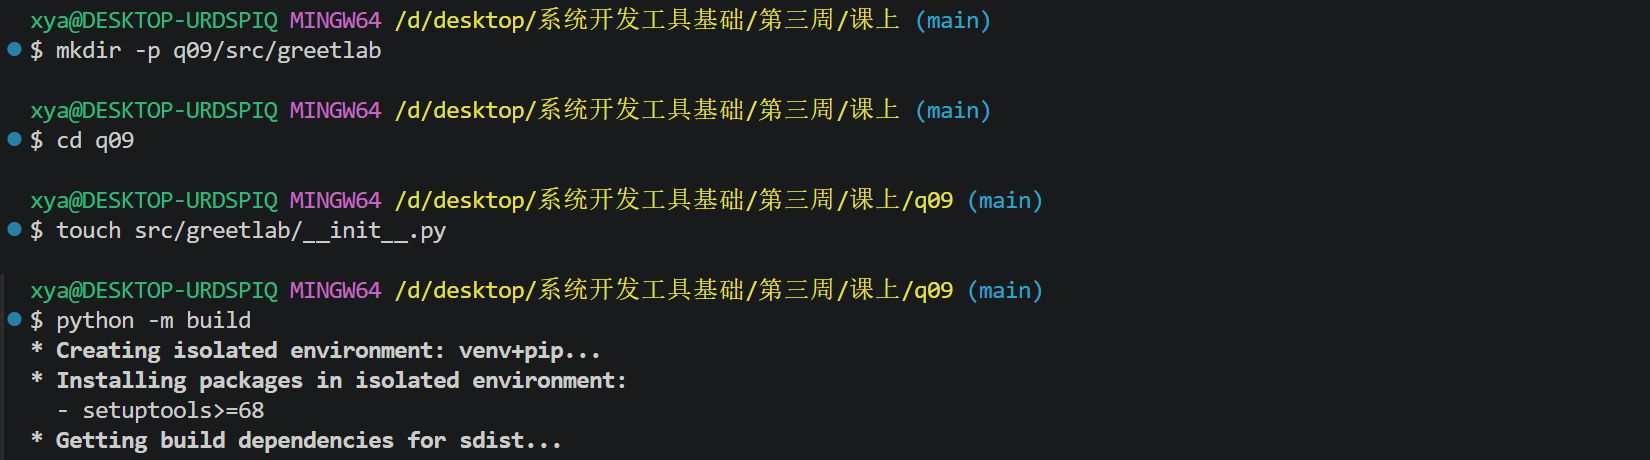
\includegraphics[width=0.96\textwidth]{课上/q09/1build省略了一大半太多了没截完整.png}\\[-0.35em]
  {\small (a) 创建包目录并开始构建}\\[-0.15em]
  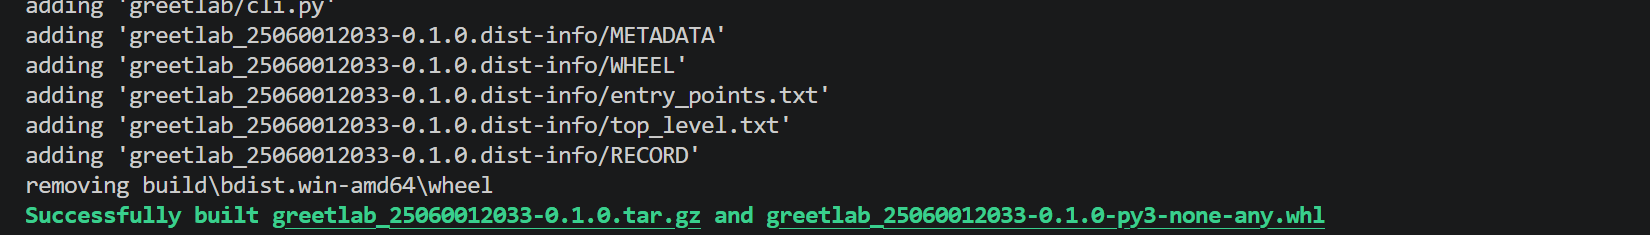
\includegraphics[width=0.96\textwidth]{课上/q09/2build结尾-中间跳过了.png}\\[-0.35em]
  {\small (b) 源码包和 wheel 构建成功}\\[-0.15em]
  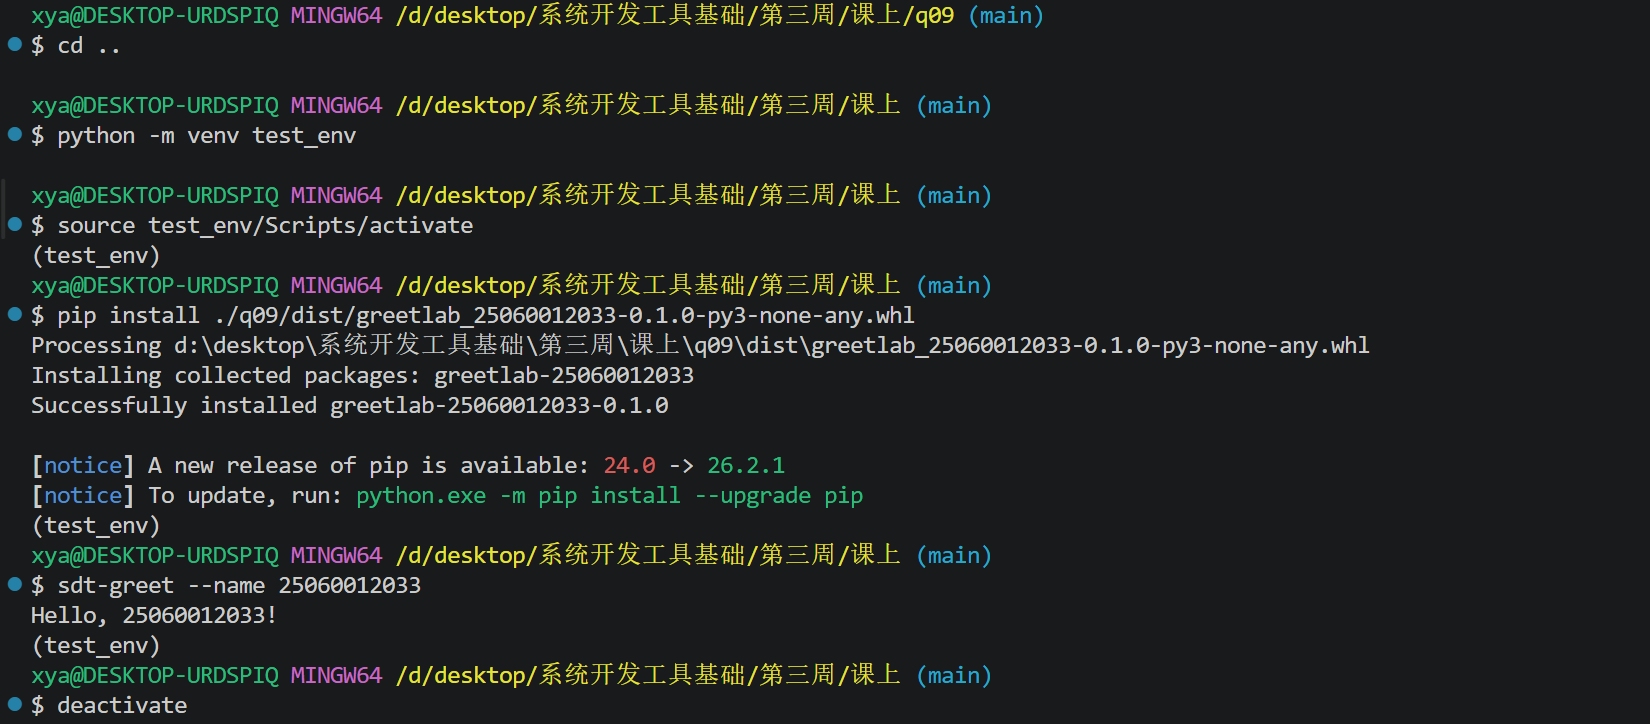
\includegraphics[width=0.96\textwidth]{课上/q09/3剩余部分.png}\\[-0.35em]
  {\small (c) 在 q09 外创建干净环境、安装 wheel 并调用命令}
  \caption{q09 从源码构建到干净环境安装验证的过程}
  \label{fig:q09-process}
\end{figure}

\textbf{实验结果：} wheel 安装后，在 q09 之外运行
\texttt{sdt-greet --name 25060012033}，终端输出
\texttt{Hello, 25060012033!}。命令行入口能够脱离源码目录运行，说明构建产物和入口配置均有效。

\FloatBarrier

% ================= q10 =================
\subsection{q10 · 让编程智能体进入可验证的修复循环（智能体编程）}

\begin{taskbox}[题目要求]
复制 q09 为 q10，使用编程智能体完成一次测试驱动修复：
\begin{itemize}[nosep]
  \item 添加失败测试，要求姓名只含空白字符时 \texttt{main} 以 \texttt{SystemExit(2)} 结束；
  \item 先运行测试确认失败，再向智能体说明目标、约束和测试命令，要求其修改实现并运行测试；
  \item 人工检查 diff，撤销无关修改并再次运行测试；
  \item 在 \texttt{ai\_log.md} 中用不超过 5 行记录核心提示、智能体改动和人工验证。
\end{itemize}
\end{taskbox}

\textbf{实验过程：} 先复制 q09，并在 \texttt{tests/test\_cli.py} 中加入正常姓名和空白姓名两个测试。
原来的 \texttt{main} 会直接打印传入内容，因此第一次运行 pytest 时正常姓名测试通过，
空白姓名测试报出 \texttt{DID NOT RAISE SystemExit}，完整失败信息见图~\ref{fig:q10-fail}。

\begin{figure}[H]
  \centering
  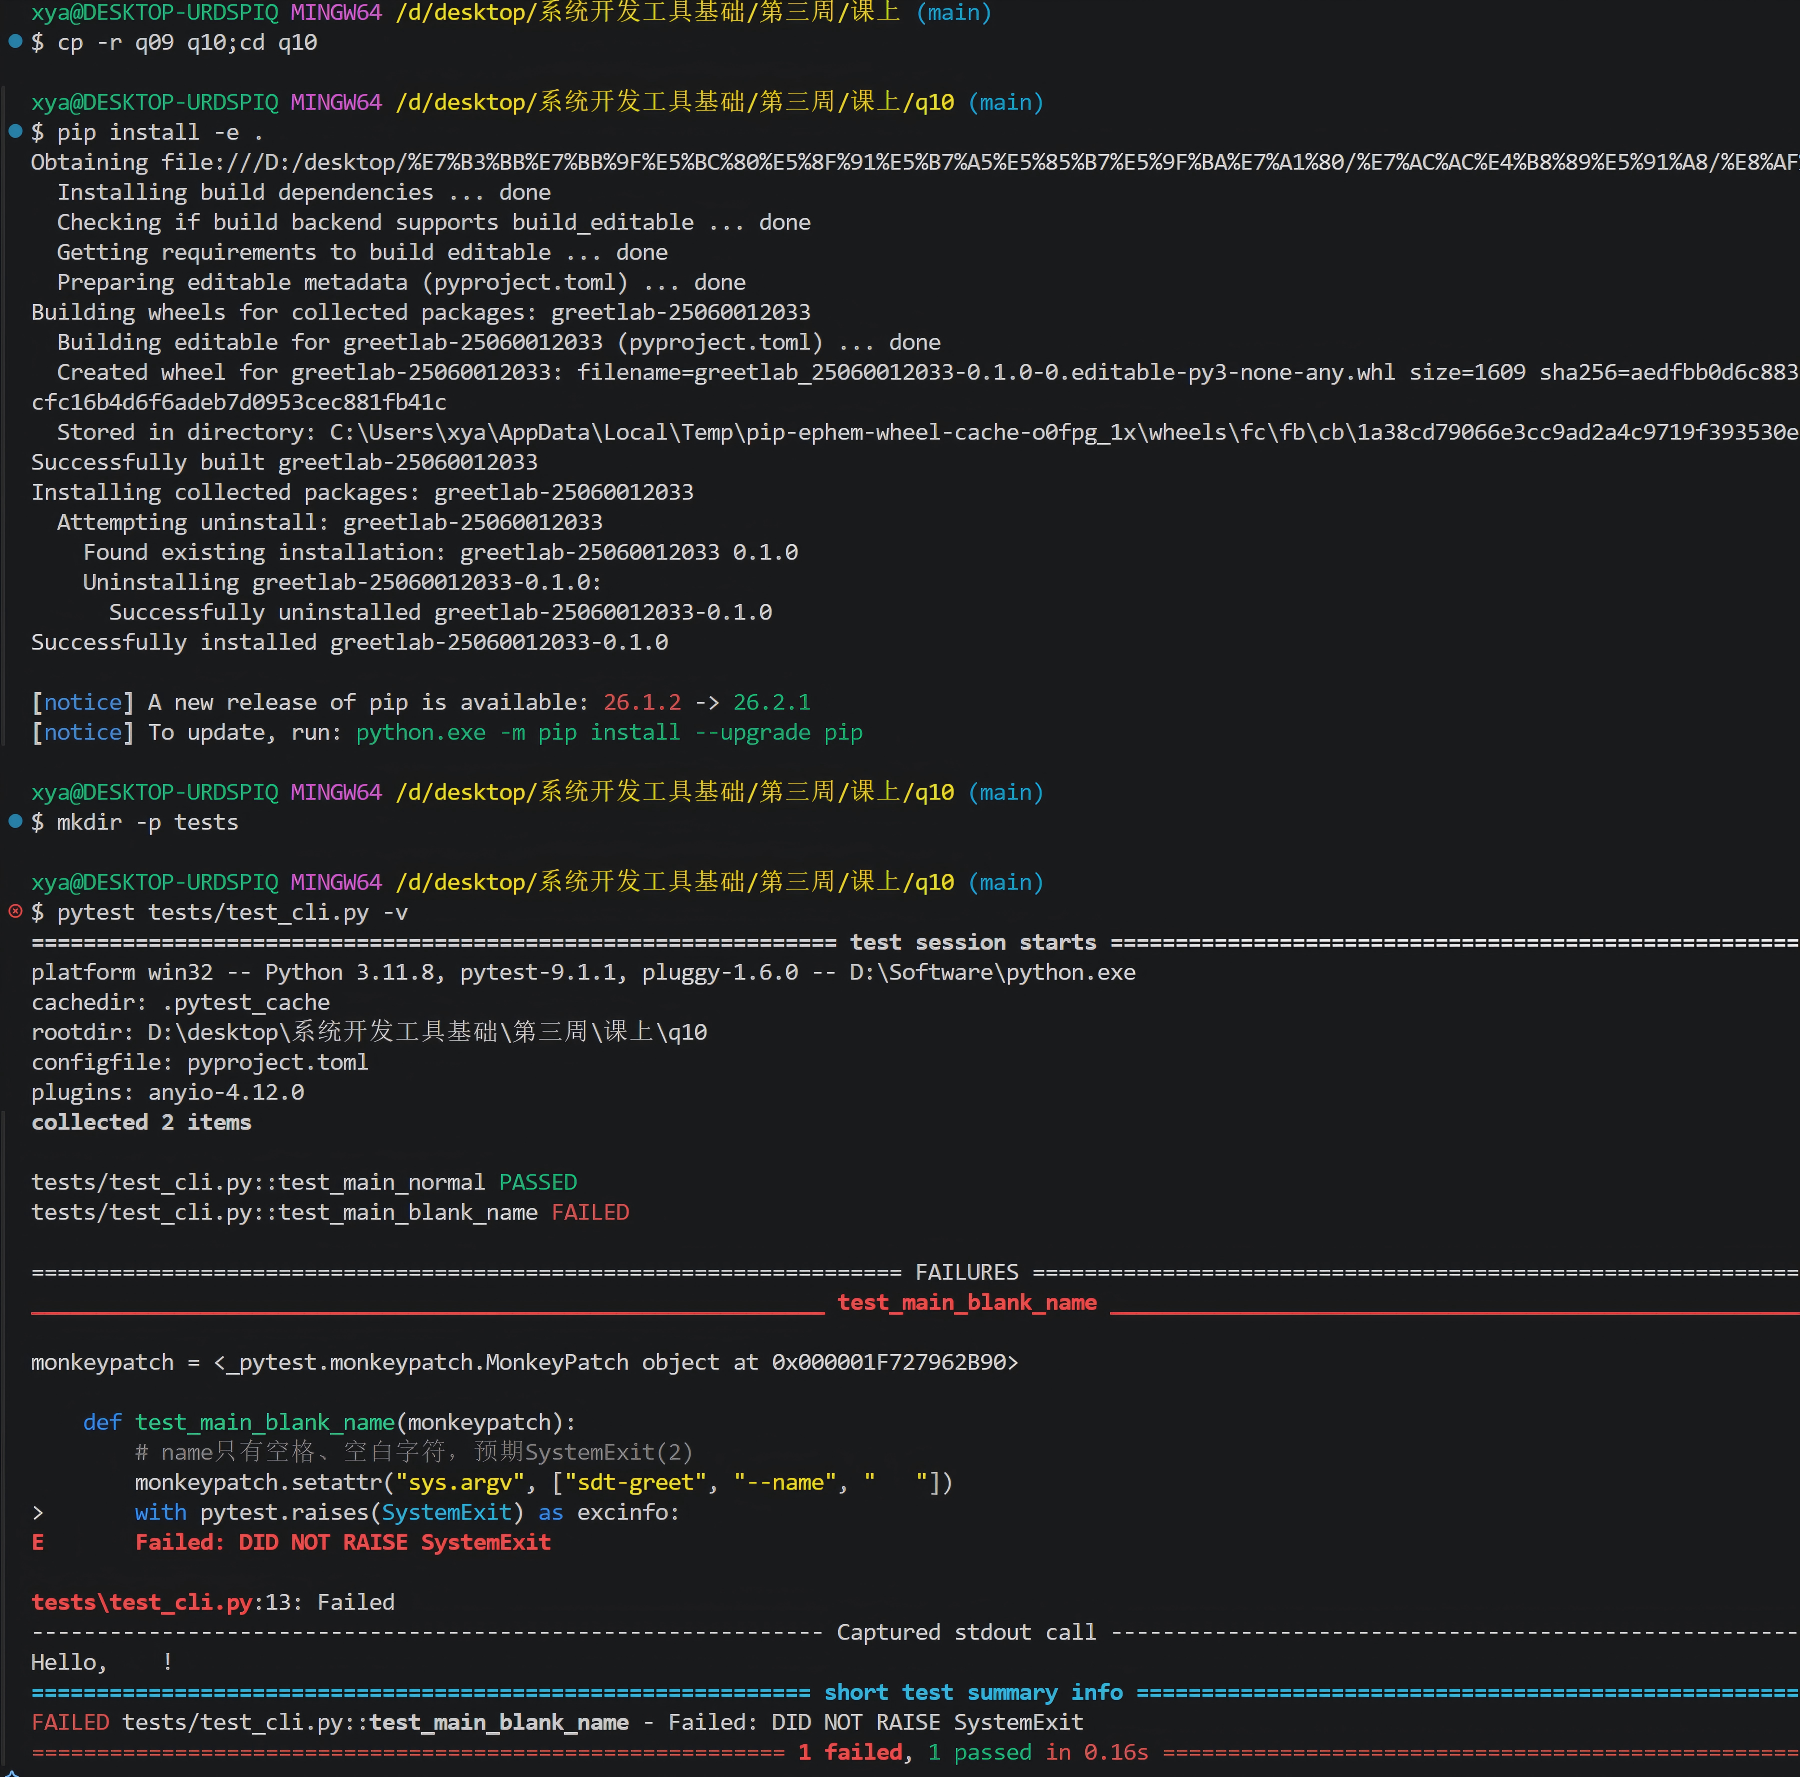
\includegraphics[trim=0 0 0 470bp,clip,width=0.96\textwidth]{课上/q10/1-agent改之前.png}
  \caption{q10 加入空白姓名测试后的首次失败结果}
  \label{fig:q10-fail}
\end{figure}

确认测试确实能暴露问题后，把失败现象、目标和限制一并交给编程智能体：只允许修改
\texttt{src/greetlab/cli.py}，禁止使用退出码不符合要求的 \texttt{p.error()}，
并给出 \texttt{pytest tests/test\_cli.py -v} 作为验证命令。智能体增加了
\texttt{name.strip()} 检查，修改内容见图~\ref{fig:q10-agent}(a)；随后由智能体运行指定测试，
两个用例均通过，见图~\ref{fig:q10-agent}(b)。

\begin{figure}[H]
  \centering
  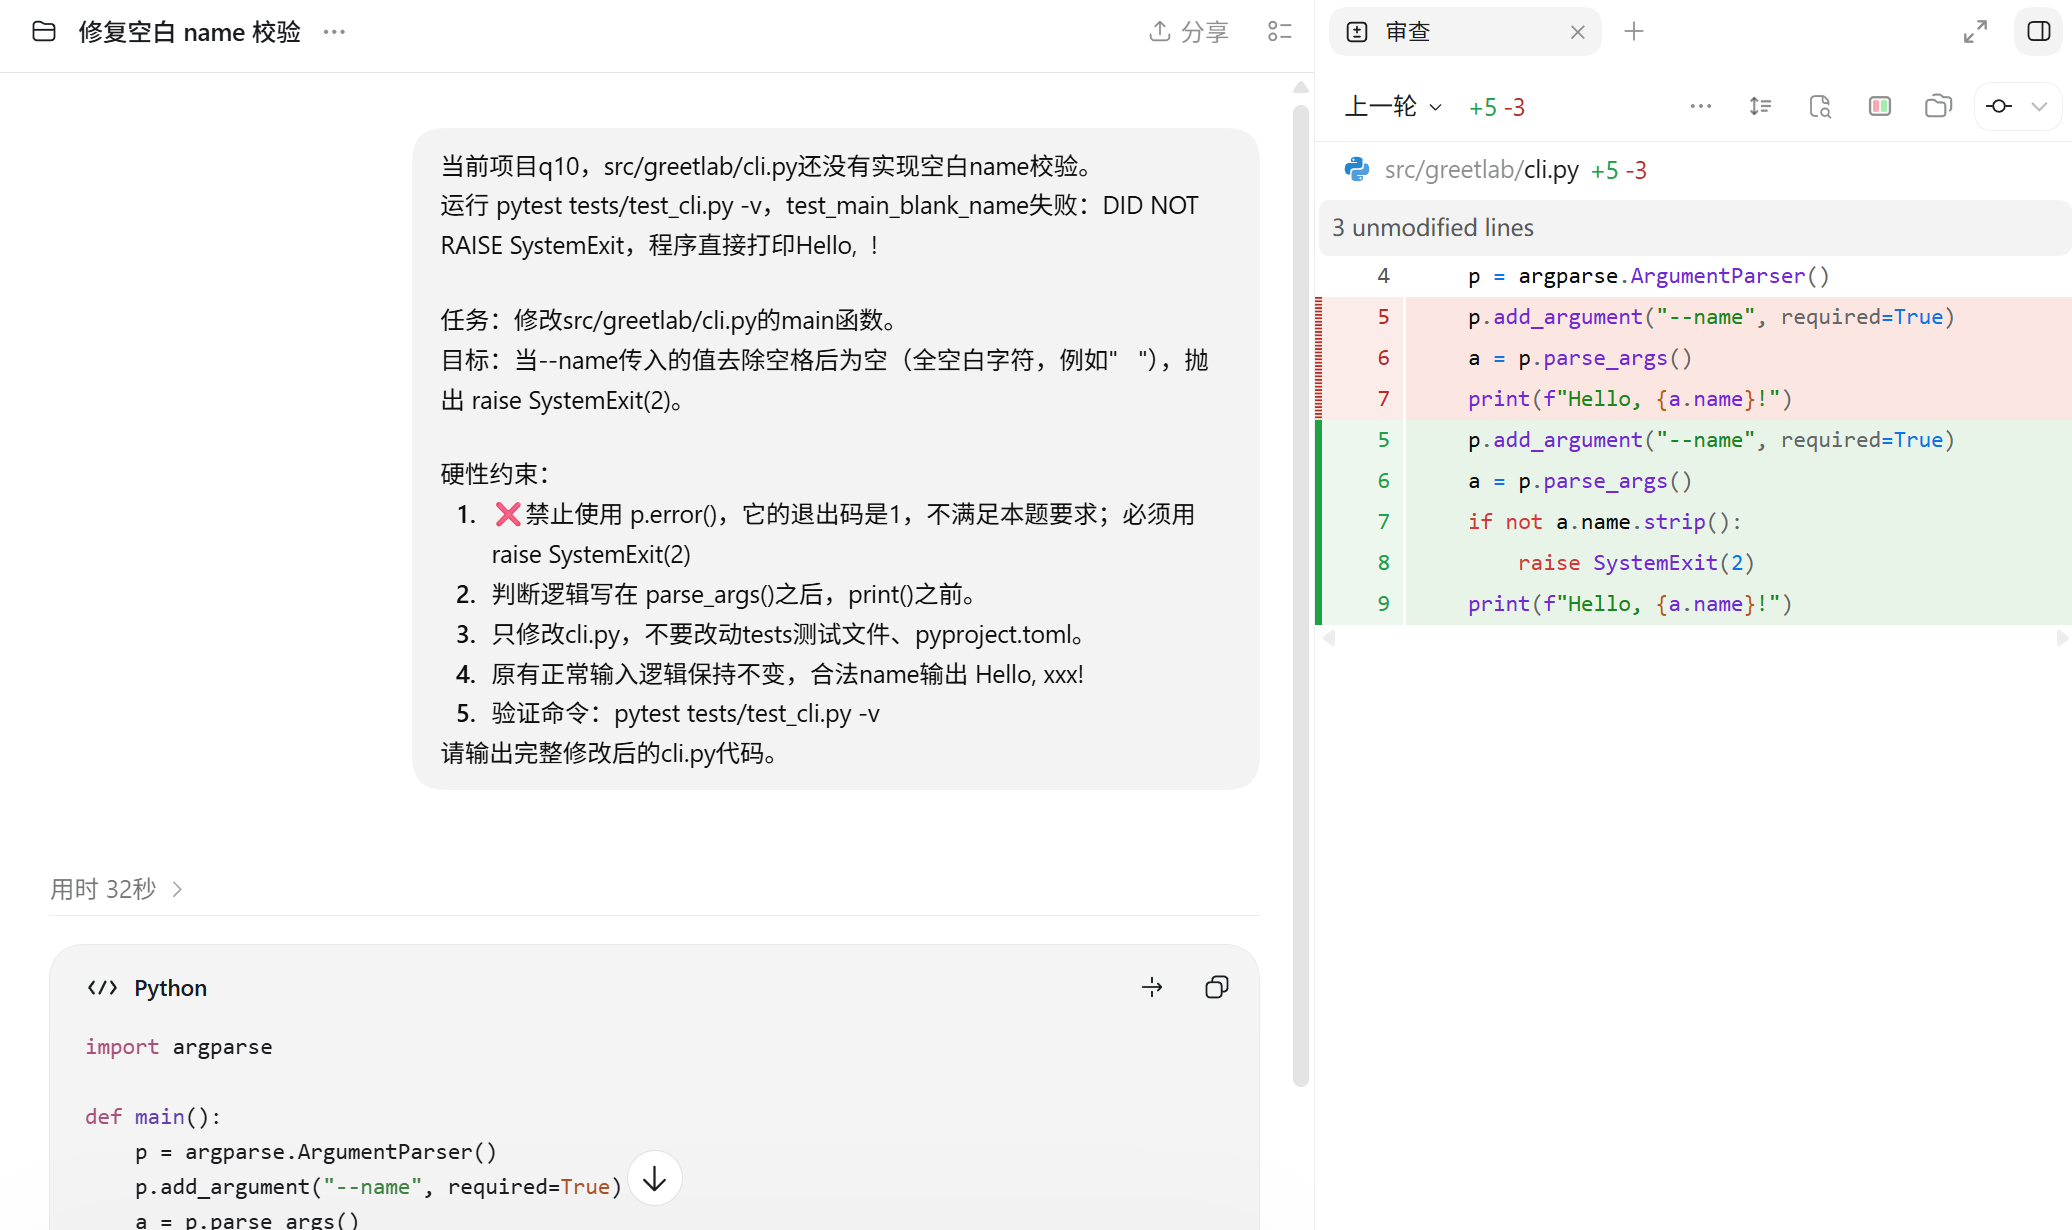
\includegraphics[width=0.90\textwidth]{课上/q10/2-agent修改.png}\\[-0.35em]
  {\small (a) 向智能体说明失败现象、修改范围和验证命令}\\[0.15em]
  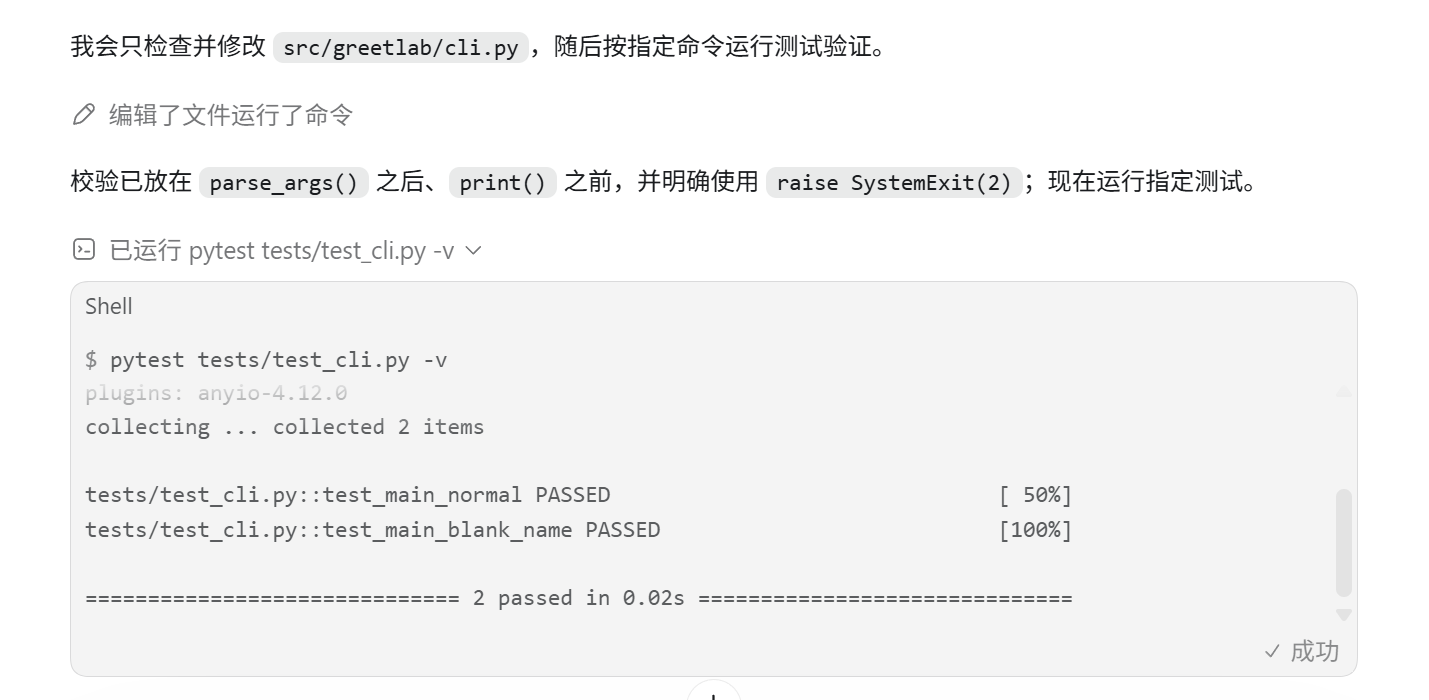
\includegraphics[width=0.90\textwidth]{课上/q10/3-agent思考过程包含测试.png}\\[-0.35em]
  {\small (b) 智能体修改后执行 pytest，两个测试通过}
  \caption{q10 编程智能体完成修改并运行测试}
  \label{fig:q10-agent}
\end{figure}

智能体修改后的实现和用于验证的测试如下。正常姓名仍输出问候语；姓名去除空白后为空时，
程序在输出前抛出 \texttt{SystemExit(2)}。

\lstinputlisting[language=py,caption={cli.py：增加空白姓名校验},label={lst:q10-cli}]{课上/q10/src/greetlab/cli.py}
\lstinputlisting[language=py,basicstyle=\footnotesize\ttfamily,caption={test\_cli.py：正常姓名与空白姓名测试},label={lst:q10-test}]{课上/q10/tests/test_cli.py}

最后人工运行 \texttt{git diff}，确认只有 \texttt{cli.py} 中与空白校验有关的修改，
再执行一次相同的 pytest 命令。终端显示两个测试均通过，耗时 0.02 s，见图~\ref{fig:q10-review}。

\begin{figure}[H]
  \centering
  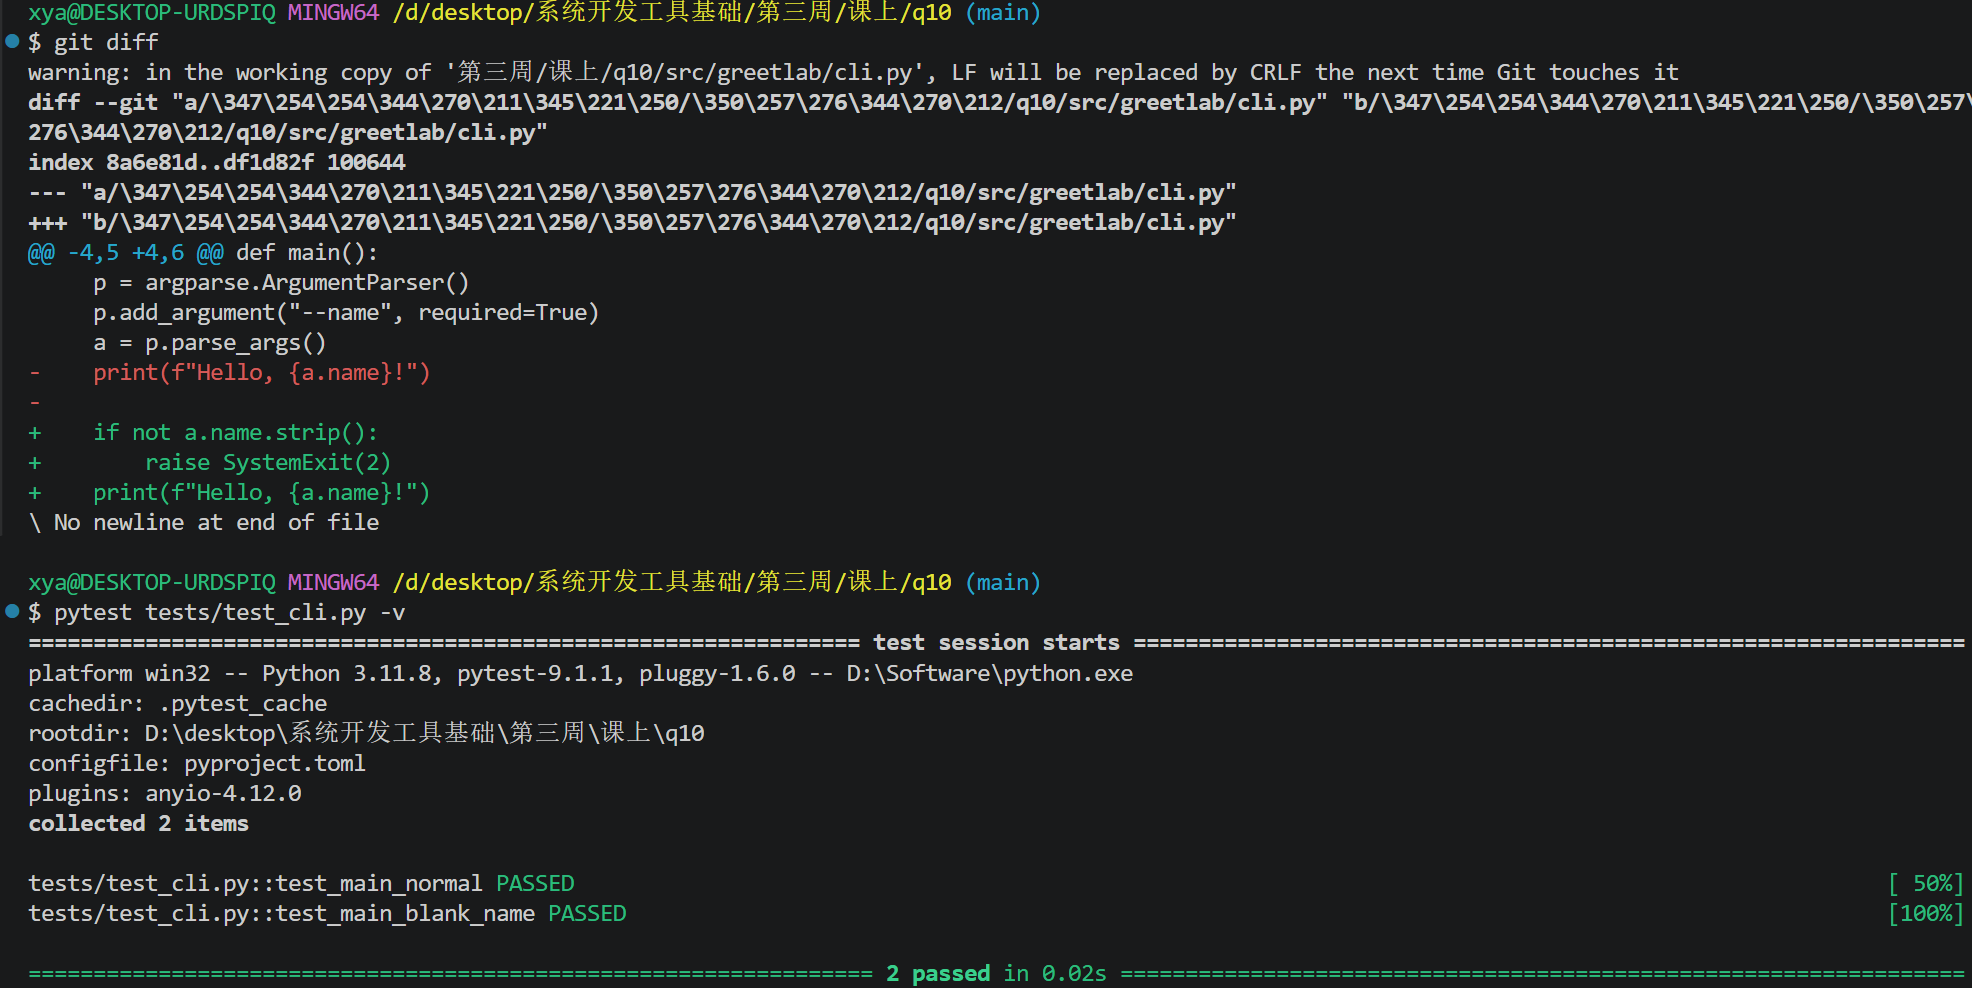
\includegraphics[width=0.96\textwidth]{课上/q10/4-giff检查以及再次测试.png}
  \caption{人工检查 diff 并再次运行测试}
  \label{fig:q10-review}
\end{figure}

修复过程记录见代码~\ref{lst:q10-ai-log}。

\lstinputlisting[language=,basicstyle=\footnotesize\ttfamily,caption={ai\_log.md：智能体修改与人工验证记录},label={lst:q10-ai-log}]{课上/q10/ai_log.md}

\textbf{实验结果：} 空白姓名现在会在打印前以状态码 2 退出，正常姓名的原有行为不变。

\FloatBarrier

% ================= q11 =================
\subsection{q11 · 把“无法处理”的协作材料改成可执行信息（不止于代码）}

\begin{taskbox}[题目要求]
围绕“空姓名仍输出问候语”这一缺陷，在 \texttt{communication.md} 中完成以下改写：
\begin{itemize}[nosep]
  \item Issue 包含环境、复现命令、期望结果和实际结果，未知信息写“待确认”；
  \item 提交信息标题使用祈使语气，正文说明问题和解决方案；
  \item 评审意见指出具体行为、风险和建议动作，并标注 Blocking、Suggestion 或 Nit；
  \item 全文控制在 400 字以内，保持专业、简洁。
\end{itemize}
\end{taskbox}

\textbf{实验过程：} 根据已知事实整理环境、复现命令和程序行为，未知版本统一标为“待确认”；
提交信息说明修改内容，评审意见用 Blocking 标出需要处理的问题。完整文件见代码~\ref{lst:q11-communication}。

\lstinputlisting[language=,basicstyle=\footnotesize\ttfamily,caption={communication.md：Issue、提交信息与评审意见},label={lst:q11-communication}]{课上/q11/communication.md}

\FloatBarrier

% ================= q12 =================
\Needspace{12\baselineskip}
\subsection{q12 · 修复一个可复现的线性回归训练循环（Python 与 PyTorch）}

\begin{taskbox}[题目要求]
补全 \texttt{q12/train.py} 并完成一次 PyTorch CPU 训练：
\begin{itemize}[nosep]
  \item 在训练循环中正确调用 \texttt{zero\_grad}、\texttt{backward} 和 \texttt{step}；
  \item 训练后调用 \texttt{model.eval()}，并在 \texttt{torch.no\_grad()} 中计算最终损失；
  \item 打印最终损失、weight 和 bias，最终损失小于 0.001；
  \item 不得直接把 weight 和 bias 赋值为 3 和 -1。
\end{itemize}
\end{taskbox}

\textbf{实验过程：} 使用题目给定的随机种子生成 101 个输入点，目标值满足
\(y=3x-1\)。模型采用单输入、单输出的 \texttt{nn.Linear}，损失函数为均方误差，
优化器为学习率 0.1 的 SGD。每轮根据当前预测计算损失，清空旧梯度后完成反向传播和参数更新，
共训练 200 轮。训练结束后切换到评估模式，并关闭梯度记录重新计算最终损失。

\lstinputlisting[language=py,basicstyle=\footnotesize\ttfamily,caption={train.py：线性回归训练与评估},label={lst:q12-train}]{课上/q12/train.py}

运行 \texttt{python train.py} 后，程序输出最终损失、weight 和 bias，结果见图~\ref{fig:q12-result}。

\begin{figure}[H]
  \centering
  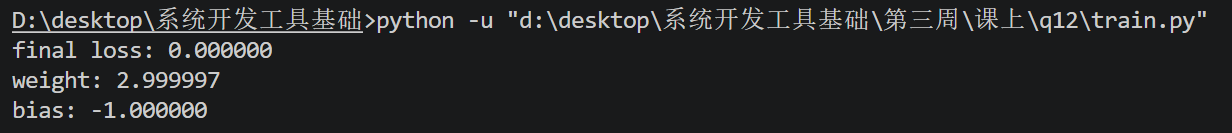
\includegraphics[width=0.96\textwidth]{课上/q12/输出结果.png}
  \caption{q12 PyTorch 线性回归的最终训练结果}
  \label{fig:q12-result}
\end{figure}

\textbf{实验结果：} 最终损失为 0.000000，weight 为 2.999997，bias 为 -1.000000，
拟合结果与目标直线 \(y=3x-1\) 一致。

\FloatBarrier

\section{课后练习}

\paragraph{参考资料记录}
\href{https://missing-semester-cn.github.io/2026/shipping-code/}{Missing Semester：Packaging and Shipping Code}、
\href{https://docs.pytorch.ac.cn/tutorials/beginner/basics/intro.html}{PyTorch 教程：学习基础知识}。

% 课后截图去掉开头的 code 命令、重复内容和无关上文，只保留运行命令与结果。
\setcounter{topnumber}{4}
\setcounter{bottomnumber}{3}
\setcounter{totalnumber}{6}
\renewcommand{\topfraction}{0.95}
\renewcommand{\bottomfraction}{0.85}
\renewcommand{\textfraction}{0.05}
\renewcommand{\floatpagefraction}{0.75}
\newcommand{\practiceimage}[5]{%
  \begin{figure}[!htbp]
    \centering
    \includegraphics[trim=#1,clip,width=#2\textwidth]{#3}
    \caption{#4}
    \label{#5}
  \end{figure}
}

\noindent\textbf{实例 1：比较虚拟环境激活前后的环境。}
先记录系统 Python、\texttt{VIRTUAL\_ENV} 和 \texttt{PATH} 的前几项，创建并激活
\texttt{.venv} 后再次记录，再用 \texttt{diff} 比较两个文件。

\begin{lstlisting}[language=shell,caption={创建虚拟环境并比较环境变化}]
python -m venv .venv
source .venv/Scripts/activate
diff -u before.txt after.txt
type deactivate | head -n 8
deactivate
\end{lstlisting}

结果见图~\ref{fig:after-1}。激活后 Python 和 \texttt{VIRTUAL\_ENV} 均指向新建的
\texttt{.venv}，虚拟环境的 \texttt{Scripts} 目录也被放到 \texttt{PATH} 前面；
\texttt{deactivate} 实际上是负责恢复原环境变量的 Shell 函数。

\practiceimage{0bp 0bp 0bp 253bp}{0.92}{课后/packaging/1.png}{虚拟环境激活前后的路径与环境变量变化}{fig:after-1}

\noindent\textbf{实例 2：检查 wheel 的内部结构。}
使用 Python 自带的 \texttt{zipfile} 模块列出并解压 q09 生成的 wheel，随后读取
\texttt{METADATA} 和 \texttt{entry\_points.txt}。

\begin{lstlisting}[language=shell,caption={列出并解压 wheel}]
python -m zipfile -l ../../../课上/q09/dist/greetlab_25060012033-0.1.0-py3-none-any.whl
python -m zipfile -e ../../../课上/q09/dist/greetlab_25060012033-0.1.0-py3-none-any.whl wheel-files
find wheel-files -type f
cat wheel-files/greetlab_25060012033-0.1.0.dist-info/METADATA
cat wheel-files/greetlab_25060012033-0.1.0.dist-info/entry_points.txt
\end{lstlisting}

图~\ref{fig:after-2} 中可以看到源码、元数据和 \texttt{RECORD} 等文件；项目名为
\texttt{greetlab-25060012033}，版本为 0.1.0，命令行入口仍指向
\texttt{greetlab.cli:main}。

\practiceimage{0bp 0bp 0bp 141bp}{0.92}{课后/packaging/2.png}{wheel 文件列表、项目元数据与命令行入口}{fig:after-2}

\noindent\textbf{实例 3：使用环境变量配置程序。}
程序通过 \texttt{os.getenv} 读取运行模式、端口和调试开关，未设置时使用开发环境默认值。

\lstinputlisting[language=py,caption={从环境变量读取运行配置},label={lst:after-config}]{课后/packaging/config-demo/config_demo.py}

直接运行时得到 \texttt{development}、8000 和 \texttt{False}；在命令前临时设置变量后，
同一份代码输出 \texttt{production}、9000 和 \texttt{True}，见图~\ref{fig:after-3}。

\practiceimage{0bp 0bp 0bp 497bp}{0.92}{课后/packaging/3.png}{默认配置与环境变量覆盖后的结果}{fig:after-3}

\noindent\textbf{实例 4：判断版本是否满足依赖约束。}
为同一组版本分别应用最低版本、范围和兼容版本三种约束，代码见代码~\ref{lst:after-version}。

\lstinputlisting[language=py,caption={使用 SpecifierSet 判断版本范围},label={lst:after-version}]{课后/packaging/version_check.py}

运行结果见图~\ref{fig:after-4}。\texttt{>=2.0} 接受 3.0.0，增加
\texttt{<3.0} 后将其排除；\texttt{\textasciitilde=2.1.0} 只匹配兼容的 2.1.5。

\practiceimage{0bp 0bp 0bp 41bp}{0.88}{课后/packaging/4.png}{三种版本约束对应的匹配结果}{fig:after-4}

\noindent\textbf{实例 5：判断 wheel 与当前解释器是否兼容。}
解析 wheel 文件名中的项目名、版本和兼容标签，再与本机 Python 支持的标签求交集。

\lstinputlisting[language=py,caption={解析并比较 wheel 兼容标签},label={lst:after-tags}]{课后/packaging/wheel_tags.py}

结果见图~\ref{fig:after-5}。该 wheel 的标签是 \texttt{py3-none-any}，兼容性判断为
\texttt{True}；本机优先标签则包含 \texttt{cp311-cp311-win\_amd64} 等 Windows 平台标签。

\practiceimage{0bp 0bp 0bp 41bp}{0.88}{课后/packaging/5.png}{wheel 标签与本机解释器标签的比较}{fig:after-5}

\noindent\textbf{实例 6：完成张量切片、矩阵乘法和拼接。}
对一个 \(2\times3\) 张量取后两列，与 \(3\times2\) 张量相乘，并沿第 0 维拼接两份原张量。

\lstinputlisting[language=py,caption={张量的切片、矩阵乘法与拼接},label={lst:after-tensor}]{课后/pytorch/tensor_ops.py}

图~\ref{fig:after-6} 中矩阵乘法得到 \(2\times2\) 结果，拼接后的形状为
\texttt{torch.Size([4, 3])}，各项结果与维度计算一致。

\practiceimage{0bp 0bp 0bp 49bp}{0.90}{课后/pytorch/1.png}{张量切片、矩阵乘法及拼接结果}{fig:after-6}

\noindent\textbf{实例 7：使用 autograd 计算梯度。}
令 \(y=x^3+2x\)，在 \(x=2\) 处反向传播；清空第一次留下的梯度后，再对
\(z=x^2\) 反向传播。

\lstinputlisting[language=py,caption={两次自动求导与梯度清零},label={lst:after-autograd}]{课后/pytorch/autograd_demo.py}

程序依次得到 (y=12)、\(\mathrm{d}y/\mathrm{d}x=14\) 和
\(\mathrm{d}z/\mathrm{d}x=4\)，与手工求导相同，见图~\ref{fig:after-7}。

\practiceimage{0bp 0bp 0bp 30bp}{0.84}{课后/pytorch/2.png}{autograd 的两次梯度计算结果}{fig:after-7}

\noindent\textbf{实例 8：使用 DataLoader 分批读取数据。}
将 10 个样本放入 \texttt{TensorDataset}，再用批大小为 4 的 \texttt{DataLoader}
按原顺序迭代。

\lstinputlisting[language=py,caption={TensorDataset 与 DataLoader 分批读取},label={lst:after-loader}]{课后/pytorch/dataloader_demo.py}

输出共包含三个批次，形状依次为 \texttt{(4,2)}、\texttt{(4,2)} 和
\texttt{(2,2)}，说明最后不足一个完整批次的数据仍被正确保留，见图~\ref{fig:after-8}。

\practiceimage{0bp 0bp 0bp 30bp}{0.86}{课后/pytorch/3.png}{DataLoader 生成的三个数据批次}{fig:after-8}

\noindent\textbf{实例 9：保存并重新加载模型参数。}
先记录随机初始化模型对固定输入的输出，再保存 \texttt{state\_dict}；新建同结构模型并加载参数后，
比较两次推理结果。完整过程见代码~\ref{lst:after-save}。

\lstinputlisting[language=py,basicstyle=\footnotesize\ttfamily,caption={保存、加载并验证模型参数},label={lst:after-save}]{课后/pytorch/save_load.py}

图~\ref{fig:after-9} 中加载前后的两个输出完全一致，\texttt{torch.allclose} 返回
\texttt{True}，生成的 \texttt{weights.pth} 大小为 2461 字节。

\practiceimage{0bp 0bp 0bp 34bp}{0.88}{课后/pytorch/4.png}{模型参数重新加载前后的输出比较}{fig:after-9}

\noindent\textbf{实例 10：构建一个多层神经网络。}
使用 \texttt{Flatten}、两个全连接层和 ReLU 组成顺序模型，并用 5 个
\(2\times2\) 样本完成一次前向计算。

\lstinputlisting[language=py,caption={顺序模型的构建与前向计算},label={lst:after-network}]{课后/pytorch/network_demo.py}

运行结果见图~\ref{fig:after-10}。输入形状为 \texttt{(5,2,2)}，展平并经过网络后输出
形状为 \texttt{(5,3)}；模型共有 67 个可训练参数。

\practiceimage{0bp 0bp 0bp 45bp}{0.90}{课后/pytorch/5.png}{网络结构、输入输出形状与参数数量}{fig:after-10}

\noindent\textbf{实例 11：计算分类概率和交叉熵损失。}
对两组三分类 logits 应用 Softmax，取最大概率对应的类别，并使用
\texttt{CrossEntropyLoss} 计算预测与标签之间的损失。

\lstinputlisting[language=py,caption={Softmax 分类概率与交叉熵损失},label={lst:after-classification}]{课后/pytorch/classification_demo.py}

如图~\ref{fig:after-11} 所示，两组概率之和均为 1，预测类别为 \texttt{[2,0]}，
与给定标签一致，交叉熵损失为 0.169846。

\practiceimage{0bp 0bp 0bp 39bp}{0.88}{课后/pytorch/6.png}{Softmax 概率、分类结果与交叉熵损失}{fig:after-11}

\FloatBarrier

\section{解题感悟}

这一周的任务感觉平时都有接触过，借此机会更好地巩固了它们。Packaging 这部分平时接触过一点，遇到问题基本就是问问ai，
虚拟环境怎么启动跟操作系统、终端都有关老是搞错路径，关于 wheel 和版本控制之前没怎么接触过，学到很多。

关于智能体编程这部分和我平时用 ai 的方式挺接近，但 q10 要求比较多，先留下失败测试，再限制只能改哪个文件，
最后还要自己看 diff 和重新跑测试。平时习惯看 ai 写的差不多能跑就用了，还是得需要注意自己检查、测试。
另外也能感觉到生产力的变化，刚进大学还是用些网页 ai ，后来接触到 agent 基本就回不去了，这也是这个时代不可逆的潮流吧。

“不止于代码”这部分刚开始感觉内容比较简单，毕竟没有多少代码要写，不过写完 Issue、提交信息和评审意见以后，
也能感觉到把问题说清楚确实能省很多事。只写一句“运行不了”基本等于还得让别人从头问一遍，环境、复现命令和实际结果
这些信息还是一次写完整比较好。

PyTorch 之前有学过一些，基本的 BP 网包括一些简单的卷积神经网络懂得原理，但是基本不会自己写代码，
都是靠智能体编程写代码。深度学习神经网络确实彻底改变了这个世界，我记得之前通识课用的时候训练很慢想用gpu训练，
结果因为 50 系列的显卡当时没有适配的 cuda ，配置各种环境配了几乎大半天，但是训练完还是很有成就感的。

这周内容跨度还是挺大的，后续也会在各种实践中继续运用到它们。

第三周课上实验、课后练习及实验报告均已提交至 Git 仓库，相关提交记录见图~\ref{fig:commit-record}。

\begin{center}
  
\includegraphics[width=\textwidth]{commit记录.png}
  \captionof{figure}{第三周实验及报告的 Git 提交记录}
  \label{fig:commit-record}
\end{center}

\end{document}
